\documentclass[10pt,a4paper]{article} % Dropped to 10pt font
\usepackage[margin=1.5cm]{geometry}   % Shaved a full cm off every margin
%% ── Packages ────────────────────────────────────────────────────────────────
\usepackage{amsmath,amssymb}
\usepackage{booktabs}
\usepackage{graphicx}
\usepackage{subcaption}
\usepackage{hyperref}
\usepackage{xcolor}
\usepackage{listings}
\usepackage{float}
\usepackage{enumitem}
\usepackage{multirow}
\usepackage{array}
\usepackage{parskip}
\usepackage{titlesec}
\usepackage{fancyhdr}
\usepackage{caption}
\usepackage[expansion=false]{microtype}

% ── Spacing compression ──────────────────────────────────────────────────────
\captionsetup{font=footnotesize,skip=2pt}
\setlist{nosep,topsep=1pt,partopsep=0pt}
\titlespacing*{\section}{0pt}{5pt plus 2pt minus 2pt}{2pt plus 1pt}
\titlespacing*{\subsection}{0pt}{3pt plus 1pt minus 1pt}{1pt plus 1pt}
\titlespacing*{\paragraph}{0pt}{2pt plus 1pt minus 1pt}{1em}
\setlength{\parskip}{1.5pt}
\setlength{\floatsep}{4pt plus 1pt minus 1pt}
\setlength{\textfloatsep}{5pt plus 1pt minus 2pt}
\setlength{\intextsep}{4pt plus 1pt minus 1pt}
\setlength{\abovecaptionskip}{2pt}
\setlength{\belowcaptionskip}{0pt}
\setlength{\abovedisplayskip}{3pt}
\setlength{\belowdisplayskip}{3pt}
\setlength{\abovedisplayshortskip}{1pt}
\setlength{\belowdisplayshortskip}{1pt}

\hypersetup{colorlinks=true, linkcolor=blue!70!black, citecolor=blue!70!black, urlcolor=blue}

\lstset{
  basicstyle=\ttfamily\small,
  breaklines=true,
  frame=single,
  backgroundcolor=\color{gray!8},
  keywordstyle=\color{blue},
  commentstyle=\color{gray},
}

\setlength{\headheight}{14.5pt}
\pagestyle{fancy}
\fancyhf{}
\chead{\small ME228 --- Fatigue Strength Prediction \& Inverse Alloy Design}
\rfoot{\thepage}

%% ── Title ───────────────────────────────────────────────────────────────────
\title{\vspace{-1em}
  \large\textbf{ME228 --- Applied Data Science and Machine Learning} --- \textit{Final Project}\\[3pt]
  \Large\textbf{Data-Driven Fatigue Strength Prediction and Inverse Alloy Design}\\[-2pt]
  \vspace{0.5cm}
  \normalsize Mixture-of-Experts Regression with Empirical Reliability \& Cost-Constrained Pareto
  \vspace{-0.5em}
}
\author{
  Rudra Khandelwal (24b2140) \quad Shourya Saxena (24b2222) \\[2pt]
  Kapidhwaj Soni (24b2214) \quad Nishit Dharamshi (24b2153)
  \vspace{-0.5em}
}

\date{}
\begin{document}
\maketitle

% ─────────────────────────────────────────────────────────────────────────────
\section{Executive Summary}
% ─────────────────────────────────────────────────────────────────────────────

Fatigue causes 80--90\,\% of mechanical failures~\cite{agrawal2014}, yet fatigue tests are destructive and slow ($>$10\textsuperscript{7} cycles). We present a complete \emph{forward + inverse} ML pipeline that, for low-alloy steels:

\begin{enumerate}[nosep]
  \item Predicts rotating-bending fatigue strength (10\textsuperscript{7} cycles, MPa) from
        chemical composition and heat-treatment parameters using a two-expert ensemble.
  \item Reports a calibrated Probability of Failure (PoF) under a user-specified applied
        stress, validated against out-of-fold (OOF) residual distribution rather than a naive
        Gaussian assumption.
  \item Inversely designs the cheapest viable alloy + heat-treatment recipe given a target
        Factor of Safety, using neighbourhood sampling, kNN data-hull filtering, and Pareto
        analysis over (cost, PoF) objectives.
\end{enumerate}

\paragraph{Headline numbers.}
On the NIMS Fatigue Strength Dataset ($N\,{=}\,437$, 26 features):
\begin{itemize}[nosep]
  \item Non-carburised regime ($N\,{=}\,389$): 5-fold CV RMSE = $19.85 \pm 2.44$\,MPa
        (leakage-free; feature selection performed per fold).
  \item Carburised regime ($N\,{=}\,48$): 5-fold CV RMSE = $40.50 \pm 13.60$\,MPa
        (leakage-free; feature selection performed per fold).
  \item Held-out 20\,\% test: NC $R^2 = 0.97$, C $R^2 = 0.86$.
  \item Three of four canonical AISI grades (4140 QT, 4340 QT, 8620 carburised) predicted
        within handbook range; AISI 1045 (plain-carbon) over-predicted, defining the
        applicability boundary.
\end{itemize}


% ─────────────────────────────────────────────────────────────────────────────
\section{Problem Statement}
% ─────────────────────────────────────────────────────────────────────────────

\subsection{Engineering Context}
Two coupled questions drive alloy selection: (1) \emph{Forward} — will this alloy survive the load? (2) \emph{Inverse} — what is the cheapest alloy meeting the safety margin? S--N curves answer (1) only for catalogued grades; (2) requires an interpolating predictive model.

\subsection{Dataset}
We use the public NIMS MatNavi Fatigue Dataset~\cite{agrawal2014}: 437 experimental records
of rotating-bending fatigue strength (10\textsuperscript{7} cycles) for low-alloy steels.
Each record carries 26 input features and one target (Fatigue, MPa):
\begin{itemize}[nosep]
  \item \textbf{Chemical composition} (9 vars): C, Si, Mn, P, S, Ni, Cr, Cu, Mo (wt\,\%).
  \item \textbf{Heat-treatment} (13 vars): normalising (NT), through-hardening (THT, THt,
        THQCr), carburising (CT, Ct), diffusion (DT, Dt), quenching (QmT), tempering (TT,
        Tt, TCr).
  \item \textbf{Mill / specimen} (4 vars): reduction ratio (RedRatio), inclusion proxies
        (dA, dB, dC).
\end{itemize}

The target distribution is \emph{strongly bimodal}: carburised steels (CT\,=\,930\,°C,
$N\,{=}\,48$) cluster between 838 and 1190\,MPa, while non-carburised samples
($N\,{=}\,389$) span 225--906\,MPa with a right-skew. This bimodality directly motivates
the architectural choice in §\ref{sec:arch}.

\begin{figure}[H]
\centering
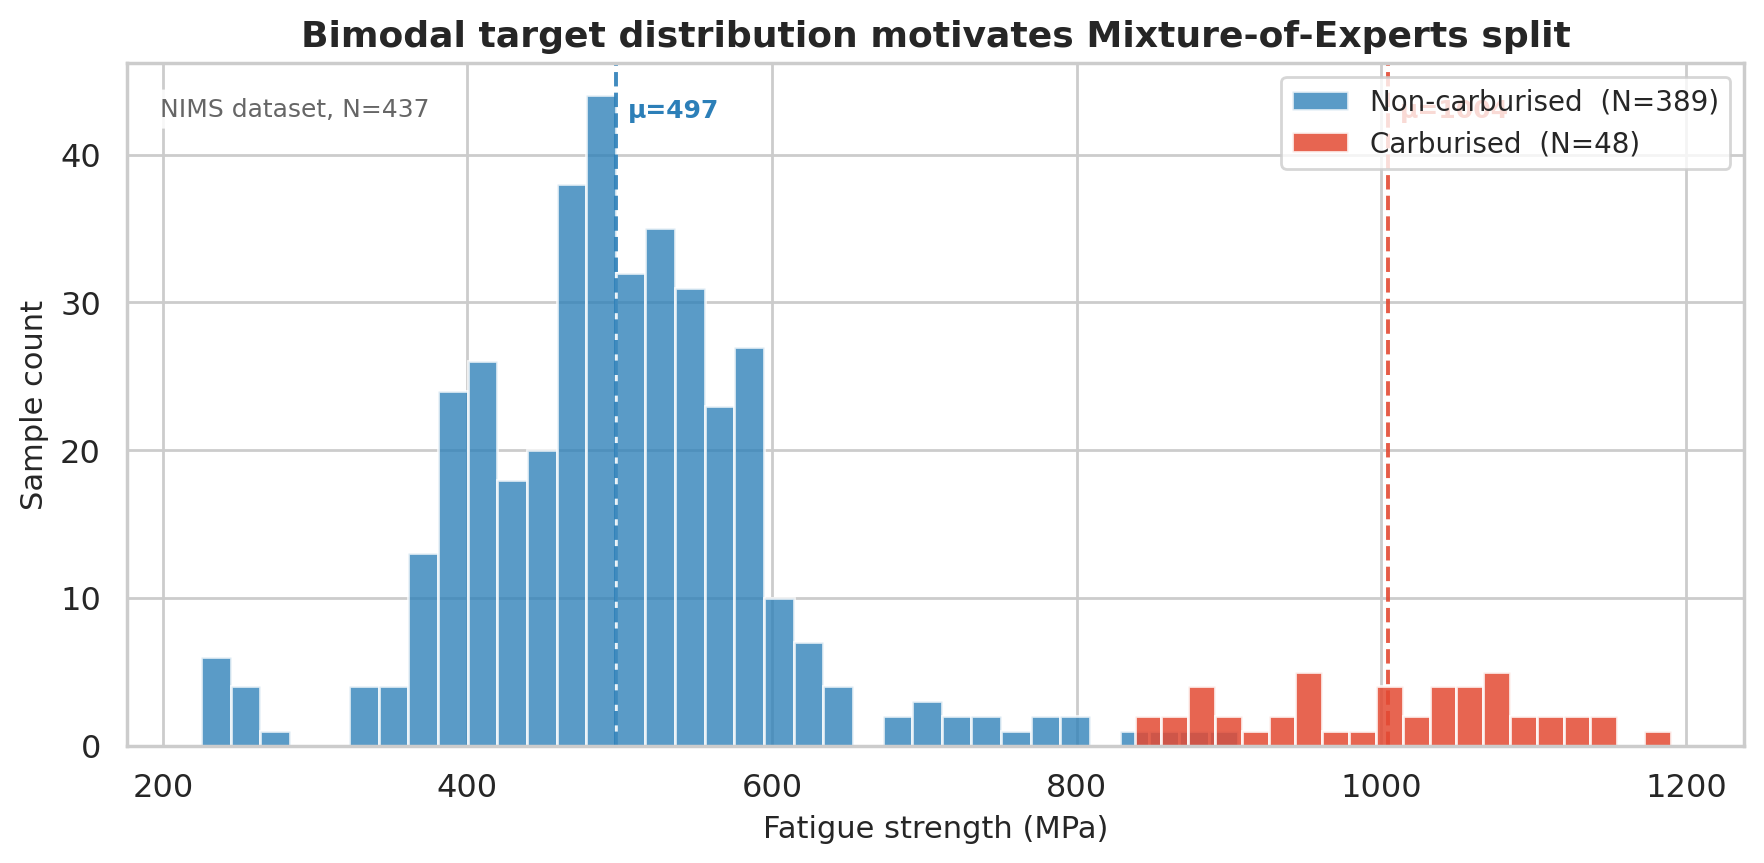
\includegraphics[width=0.62\textwidth]{slides_plots/01_bimodality.png}
\caption{NIMS fatigue distribution ($N=437$). Bimodal: NC ($\mu=497$\,MPa, blue) vs.\ carburised ($\mu\approx1007$\,MPa, red). Gap $>$250\,MPa motivates separate experts.}
\label{fig:bimodal}
\end{figure}

\subsection{Applicability Boundary}
The model is restricted to alloyed steels (Cr+Ni+Mo\,$\geq$\,0.1\,wt\%); plain-carbon grades (e.g.\ AISI 1045) are over-predicted (§\ref{sec:ext}).


% ─────────────────────────────────────────────────────────────────────────────
\section{Final Architecture}\label{sec:arch}
% ─────────────────────────────────────────────────────────────────────────────

\begin{figure}[H]
\centering
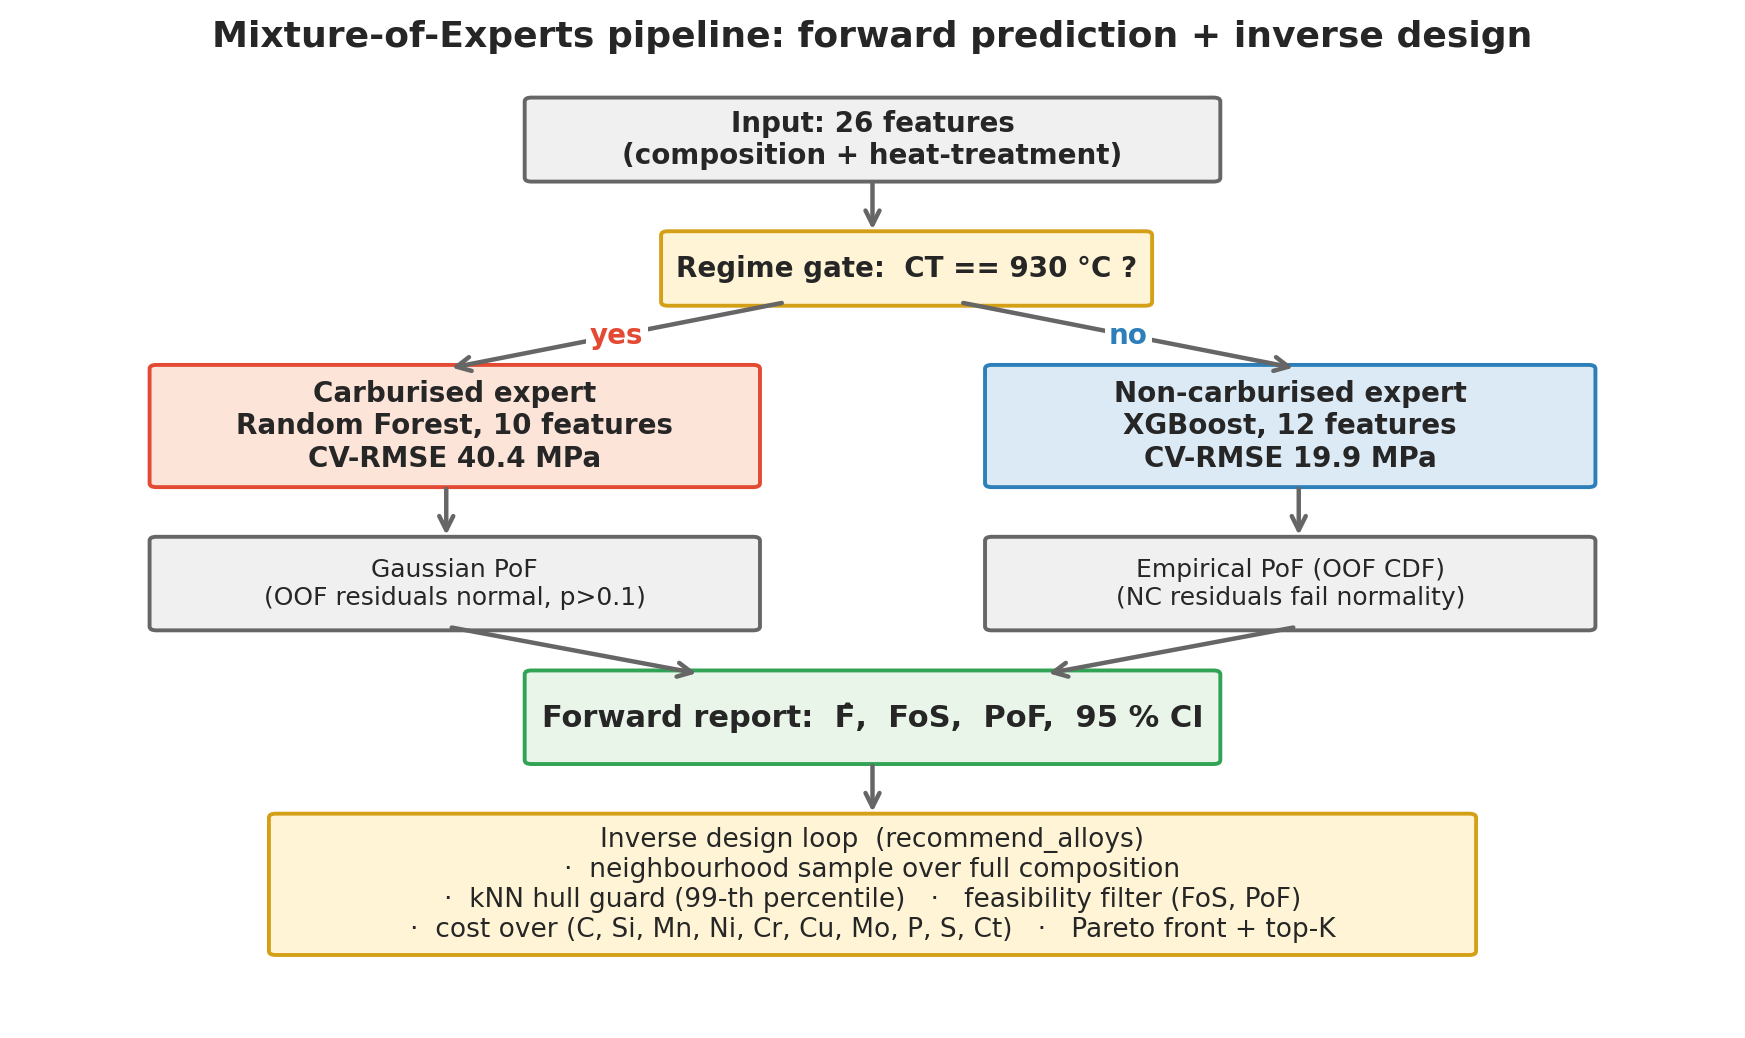
\includegraphics[width=0.78\textwidth]{slides_plots/02_architecture.png}
\caption{Pipeline. Gate ($CT=930\,^\circ$C) routes to NC expert (XGBoost, 12 feat, 19.9\,MPa) or C expert (RF, 10 feat, 40.5\,MPa). Both feed forward report and inverse design.}
\label{fig:arch}
\end{figure}

\subsection{Why Mixture-of-Experts (MoE)}\label{sec:moe}
A single global model averages two physically distinct strengthening mechanisms
(case-hardening vs.\ through-hardening) and produces an inflated, regime-blind error.
We engineer a binary gate
\[
  \texttt{is\_carburized} = \mathbf{1}[\,CT = 930\,]
\]
and route to two independent experts.

\textbf{Note.} A tuned global XGBoost achieves the same pooled RMSE (23.1\,MPa) as the MoE. The MoE wins on \emph{regime-specific calibration}: each expert has its own residual distribution and $\sigma$, essential for trustworthy PoF.

\subsection{Per-regime Model Choice}
We benchmark four candidate model families on the regime-specific features under
5-fold cross-validation, using default hyperparameters to isolate the effect of model
class:

\begin{table}[H]
\centering
\caption{Untuned 5-fold CV RMSE per regime. Bold = chosen family.}
\label{tab:benchmark}
\begin{tabular}{lrr}
\toprule
\textbf{Model} & \textbf{NC RMSE (MPa)} & \textbf{C RMSE (MPa)} \\
\midrule
\textbf{XGBoost} & \textbf{23.47 ± 1.77} & 59.42 ± 15.90 \\
\textbf{Random Forest} & 25.76 ± 1.81 & \textbf{46.33 ± 10.69} \\
Ridge            & 36.53 ± 1.29 & 75.81 ± 21.00 \\
kNN ($k=7$)      & 70.98 ± 8.42 & 73.73 ± 2.48 \\
\bottomrule
\end{tabular}
\end{table}

\textbf{NC (XGBoost).} Tuned XGBoost reaches 19.9\,MPa, the lowest CV-RMSE in the
benchmark. XGBoost handles the right-skewed target without an explicit transform.

\textbf{C (Random Forest).} With $N\,{=}\,48$, RF's bagging and aggressive depth-limit make
it strictly more robust than XGBoost's boosting cascade. Tuned RF: 40.5\,MPa.

\begin{figure}[H]
\centering
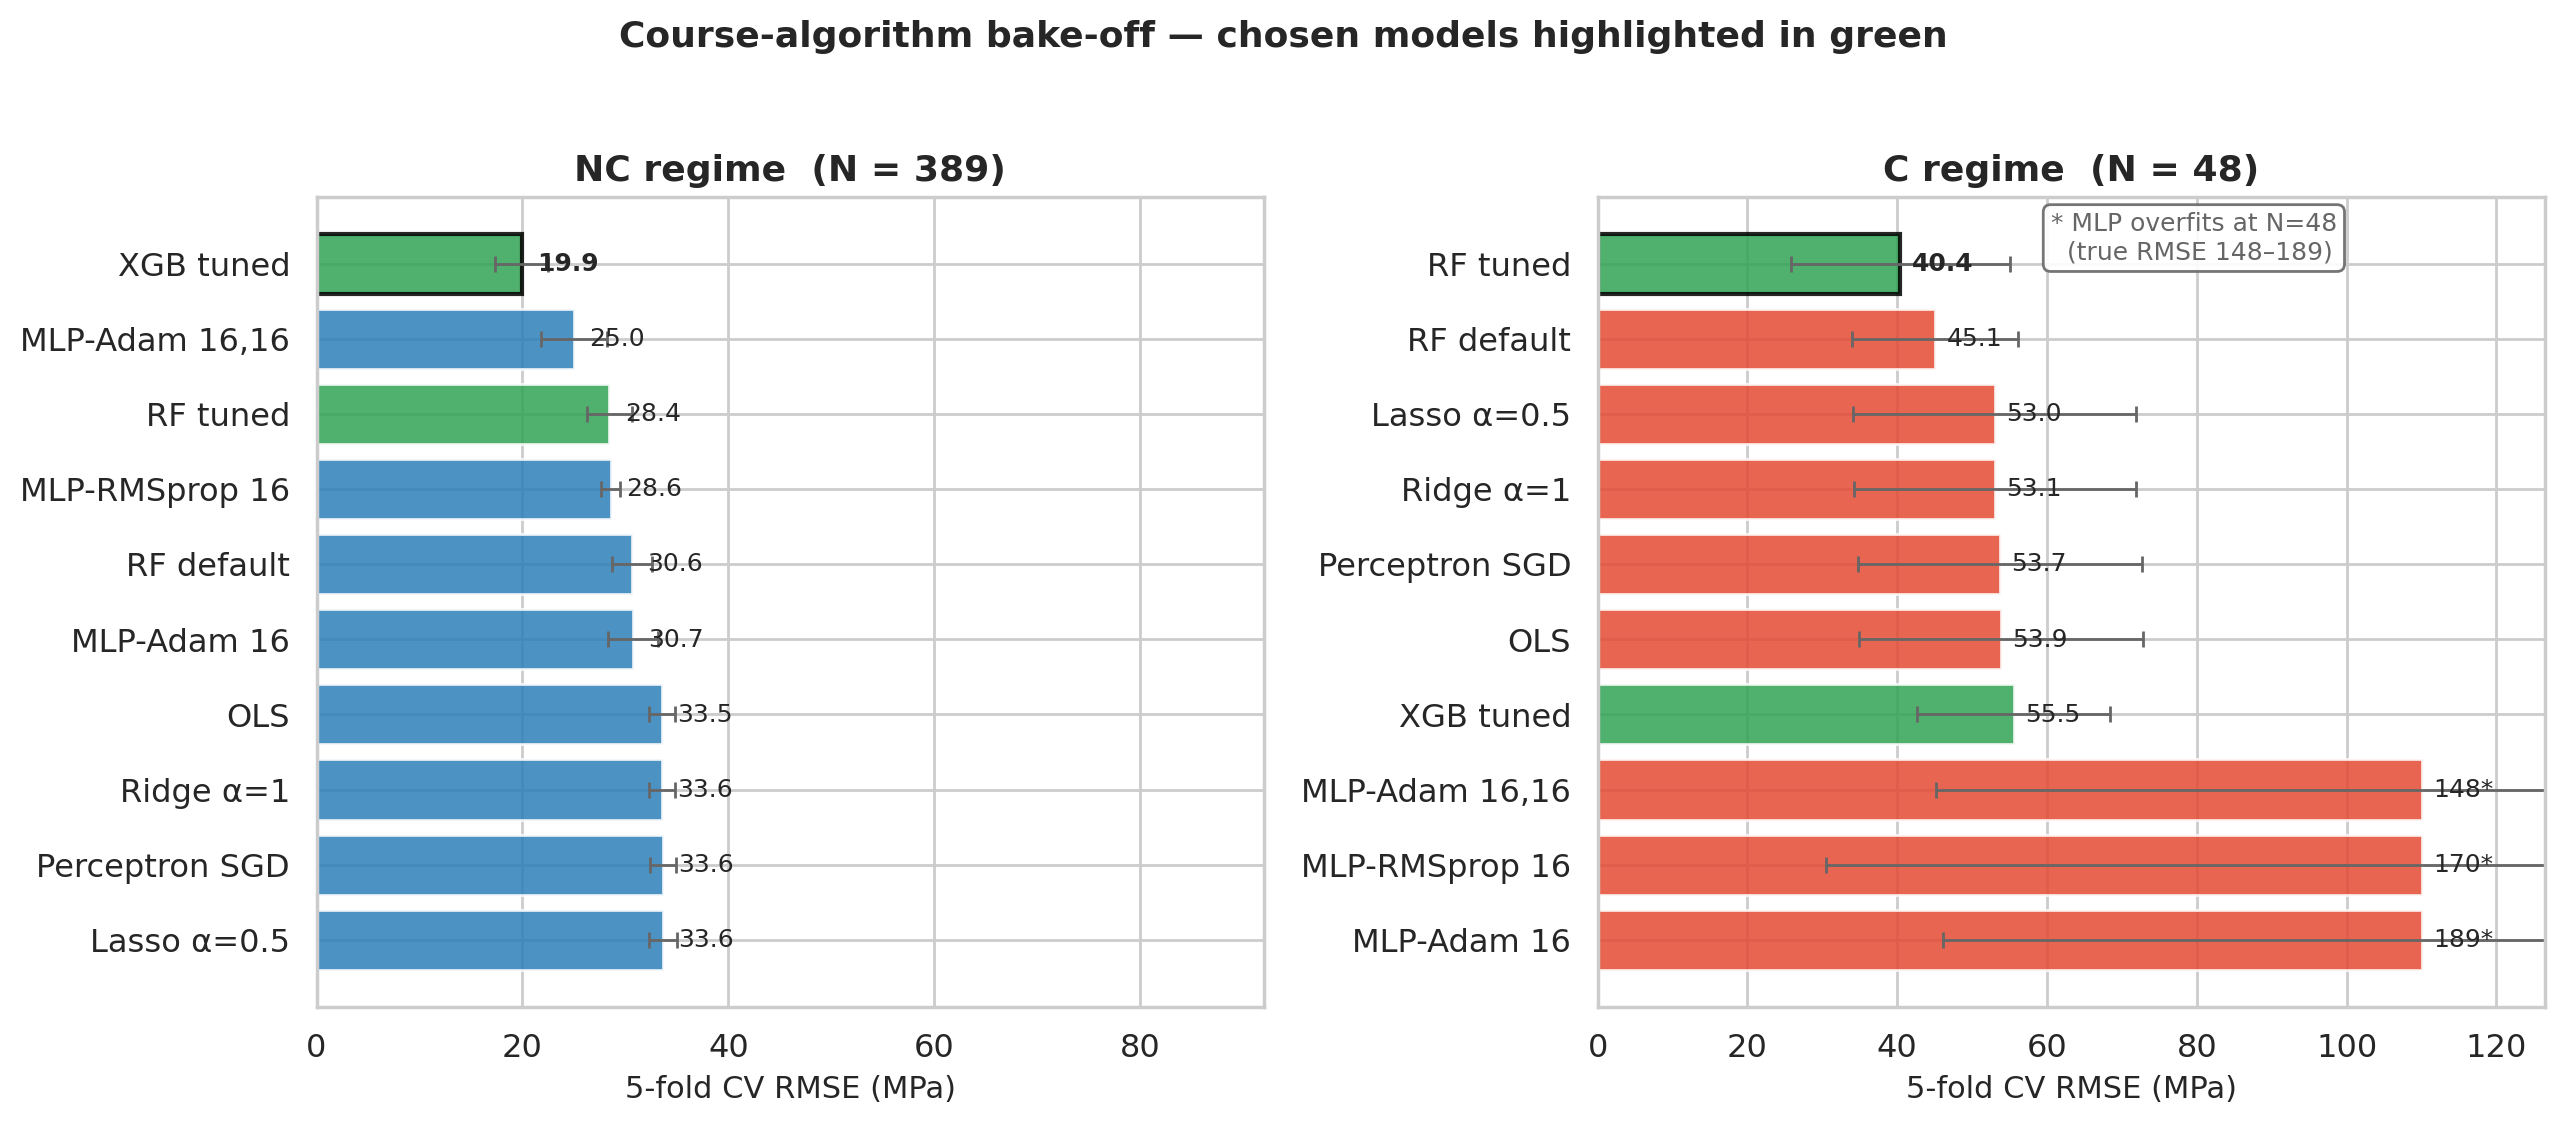
\includegraphics[width=0.70\textwidth]{slides_plots/03_bakeoff.png}
\caption{5-fold CV RMSE per regime (chosen models in green). NC: XGBoost 19.9\,MPa leads; MLPs overfit. C: RF 40.5\,MPa leads; deep MLPs 148--189\,MPa.}
\label{fig:benchmark}
\end{figure}

\subsection{Feature Selection \texorpdfstring{(VIF $\rightarrow$ SHAP)}{(VIF to SHAP)}}
The 26 raw features contain heavy collinearity (e.g.\ CT, DT, QmT all encode the same
thermal cycle). We apply a two-stage reduction:
\begin{enumerate}[nosep]
  \item \textbf{VIF filter:} iteratively drop the feature with the largest variance
        inflation factor until all VIF\,$<$\,10. Drops 6 features per regime.
  \item \textbf{SHAP scout:} fit a shallow Random Forest on VIF survivors and retain the
        top-$k$ features by mean $|\,\text{SHAP}\,|$. $k=12$ for NC, $k=10$ for C.
\end{enumerate}

\paragraph{No data leakage.} Both stages are encapsulated in \texttt{VIFThenShapSelector} (a custom \texttt{sklearn} transformer) and composed into a \texttt{Pipeline}. Under \texttt{cross\_val\_score}, VIF and SHAP-scout re-fit on each training fold only; held-out folds never influence feature selection. The CV-RMSEs ($19.85 \pm 2.44$\,MPa NC, $40.50 \pm 13.60$\,MPa C) are leakage-free. Final feature lists are extracted from a full-data fit \emph{after} CV, solely for deployment.

\begin{table}[H]
\centering
\caption{Final selected features per regime.}
\label{tab:features}
\begin{tabular}{ll}
\toprule
\textbf{Regime} & \textbf{Selected features} \\
\midrule
Non-carburised & Cr, TT, C, Mn, THT, Mo, Si, RedRatio, P, S, dA, Cu \\
Carburised     & P, RedRatio, Ct, Mo, S, Mn, Cu, Dt, TT, QmT \\
\bottomrule
\end{tabular}
\end{table}

\paragraph{Physical interpretation.} NC: TT and Cr dominate (martensite tempering). C: Ct, RedRatio, Mo dominate; bulk C drops out because case carbon is set by the carburising atmosphere.

\subsection{Hyperparameter Tuning}
Optuna TPE search, 60 trials, with 5-fold CV as the objective.

\begin{table}[H]
\centering
\caption{Best hyperparameters from Optuna.}
\label{tab:hparams}
\begin{tabular}{lll}
\toprule
\textbf{Parameter} & \textbf{NC XGBoost} & \textbf{C Random Forest} \\
\midrule
n\_estimators       & 396                 & 313 \\
max\_depth          & 4                   & 9 \\
learning\_rate      & 0.085               & --- \\
subsample           & 0.924               & --- \\
colsample\_bytree   & 0.640               & --- \\
min\_child\_weight  & 4                   & --- \\
reg\_alpha          & 1.83                & --- \\
reg\_lambda         & 0.015               & --- \\
min\_samples\_split & ---                 & 9 \\
min\_samples\_leaf  & ---                 & 2 \\
max\_features       & ---                 & 0.927 \\
\bottomrule
\end{tabular}
\end{table}


% ─────────────────────────────────────────────────────────────────────────────
\section{Reliability: Empirical PoF}\label{sec:reliability}
% ─────────────────────────────────────────────────────────────────────────────

The deployment wrapper maps a prediction to a Probability of Failure under applied stress
$\sigma_{\text{app}}$:
\[
  \text{PoF} = P(F < \sigma_{\text{app}})
\]
where $F$ is the realised fatigue strength of a fresh specimen.

\subsection{Limitations of the Gaussian Assumption}
A first-pass approach uses
$\text{PoF} = \Phi\!\big((\sigma_{\text{app}} - \hat{F}) / \sigma_{\text{CV}}\big)$.
This is correct only when the residuals $r = F - \hat{F}$ are Gaussian.

\textbf{Test on OOF residuals}: Training-fit residuals are optimistically biased; we test on out-of-fold (OOF) residuals instead.

\begin{table}[H]
\centering
\caption{Residual normality on OOF predictions vs.\ training fit.}
\label{tab:residuals}
\setlength{\tabcolsep}{5pt}
\begin{tabular}{l l r p{3.4cm} r r}
\toprule
\textbf{Regime} & \textbf{Source} & \textbf{Std (MPa)}
                & \textbf{Range (MPa)} & \textbf{Shapiro $p$} & \textbf{KS $p$} \\
\midrule

NC & Train fit            &  5.28 & $-33.7$ to $+26.6$    & 0.0000 & 0.2970 \\
NC & \textbf{OOF}         & \textbf{19.65} & \textbf{$-104.9$ to $+109.9$}
                                                           & \textbf{0.0000} & \textbf{0.0007} \\
C  & Train fit            & 30.14 & $-79.1$ to $+61.2$    & 0.3393 & 0.7305 \\
C  & \textbf{OOF}         & \textbf{43.18} & \textbf{$-110.5$ to $+87.2$}
                                                           & 0.3747 & 0.5921 \\
\bottomrule
\end{tabular}
\end{table}

\textbf{Conclusion.}
\begin{itemize}[nosep]
  \item NC OOF residuals fail \emph{both} normality tests ($p < 0.001$) — heavy right tail.
        Gaussian PoF is invalid; we use the empirical CDF.
  \item C OOF residuals pass both tests; Gaussian PoF is valid.
\end{itemize}

\begin{figure}[H]
\centering
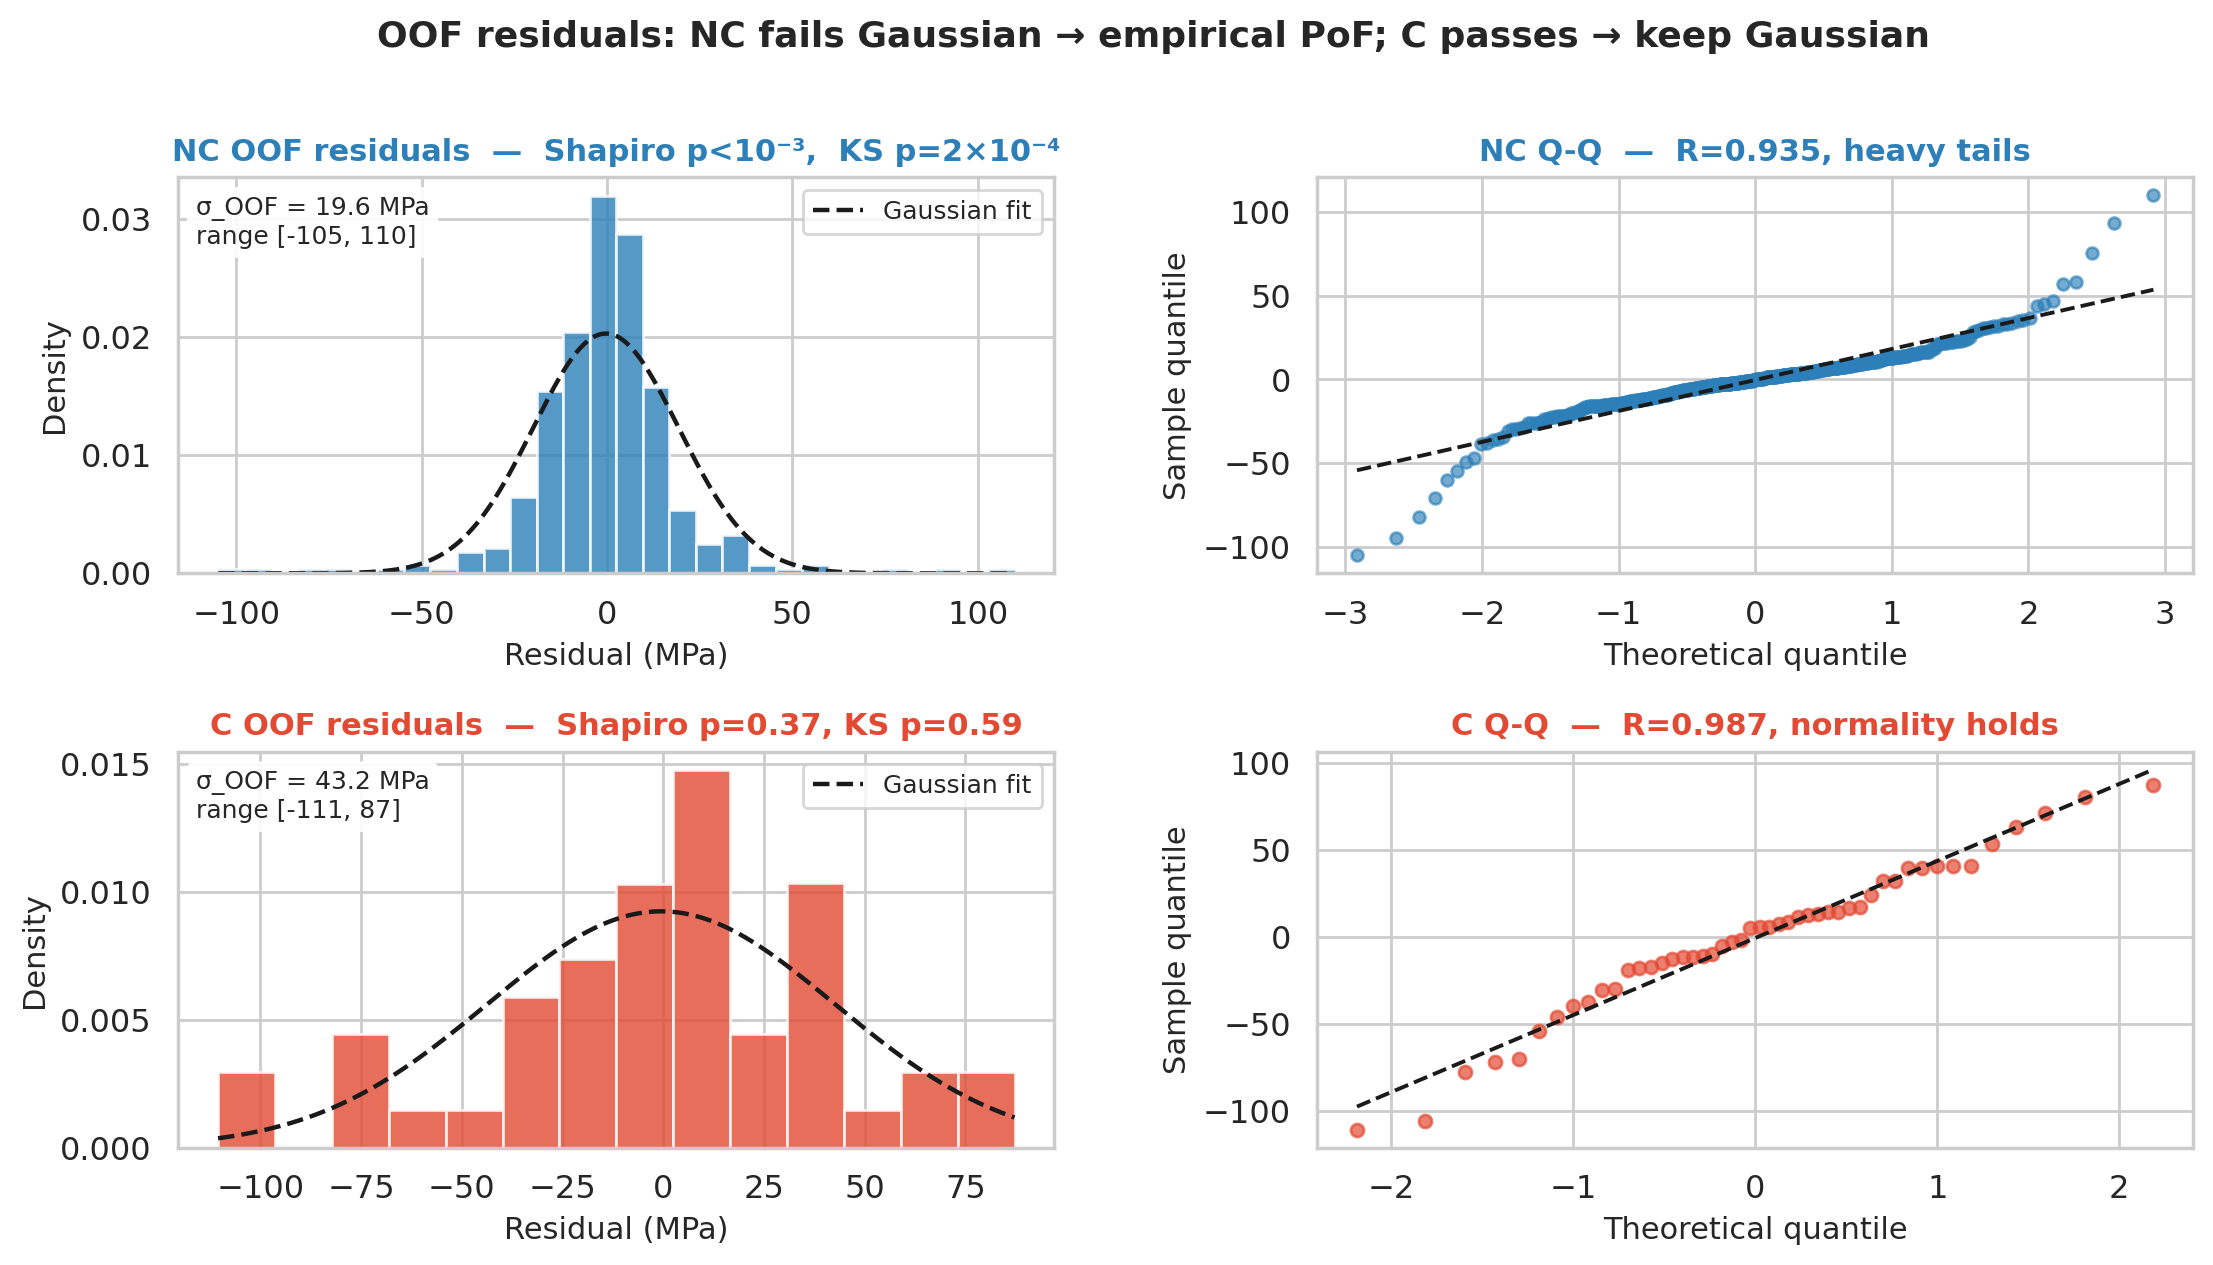
\includegraphics[width=0.68\textwidth]{slides_plots/04_oof_residuals.png}
\caption{OOF residual diagnostics. NC (top): heavy tails, Shapiro $p<10^{-3}$ — empirical CDF required. C (bottom): normal ($p=0.37$) — Gaussian PoF valid.}
\label{fig:oof}
\end{figure}

\subsection{Empirical PoF Formula (NC)}
We pre-compute OOF residuals $\{r_i\}_{i=1}^{389}$ at startup. For a candidate with
predicted fatigue $\hat{F}$ at applied stress $\sigma_{\text{app}}$:
\[
  \text{PoF}_{\text{empirical}}
    = P(\hat{F} + r < \sigma_{\text{app}})
    = \frac{1}{389}\sum_{i=1}^{389}\mathbf{1}\!\left[r_i < \sigma_{\text{app}} - \hat{F}\right].
\]
This is the empirical CDF of residuals evaluated at the gap. It captures heavy tails and
asymmetry that $\Phi$ misses.

\paragraph{Magnitude of the correction.}
At $\sigma_{\text{app}} = 590$\,MPa, $\hat{F} = 585.0$\,MPa:
$\text{PoF}_{\text{Gaussian}} = 0.600$ vs.\ $\text{PoF}_{\text{empirical}} = 0.666$ — 6.5\,pp difference. Gaussian is over-confident in the upper tail; at low applied stresses the discrepancy reverses and collapses at large margins.

\begin{figure}[H]
\centering
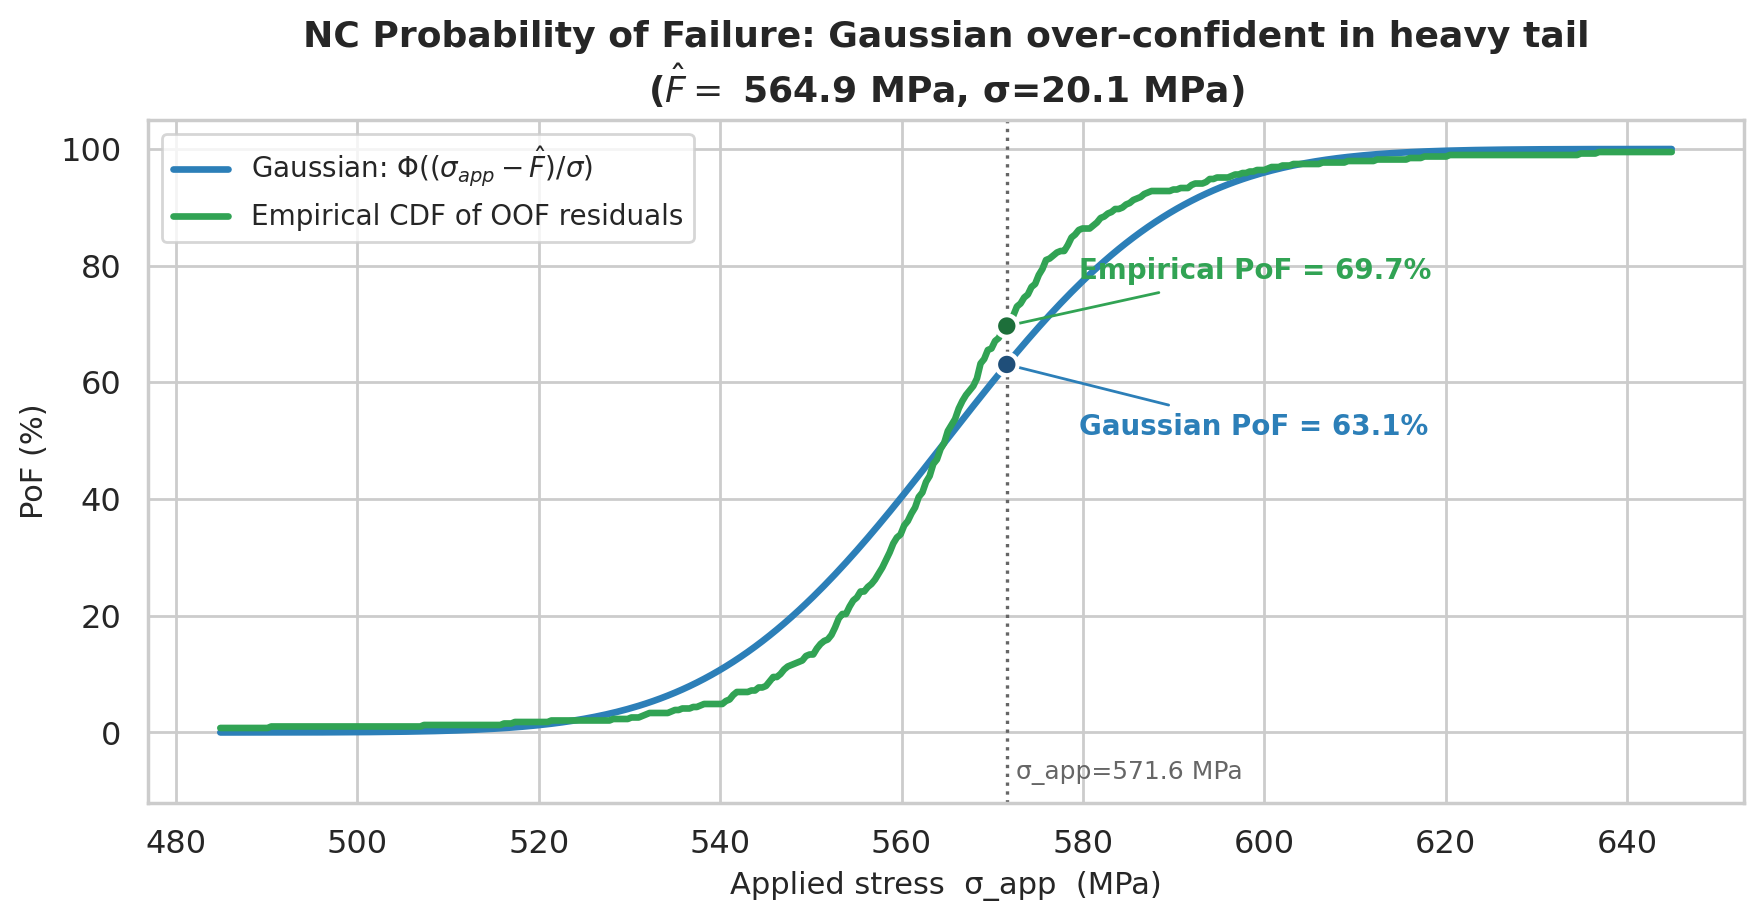
\includegraphics[width=0.58\textwidth]{slides_plots/05_pof_compare.png}
\caption{NC PoF curves ($\hat{F}=585.0$\,MPa). At $\sigma_{\text{app}}=590$\,MPa: Gaussian 60.0\,\% vs.\ empirical 66.6\,\% (+6.5\,pp). Gap vanishes at large safety margins.}
\label{fig:pof}
\end{figure}


% ─────────────────────────────────────────────────────────────────────────────
\section{Inverse Design}
% ─────────────────────────────────────────────────────────────────────────────

Given $\sigma_{\text{app}}$, target Factor of Safety FoS$^*$, and PoF cap $\tau$, find the
cheapest alloy $\mathbf{x}^*$ that satisfies:
\begin{align}
  \hat{F}(\mathbf{x}^*) &\geq \text{FoS}^* \cdot \sigma_{\text{app}}, \label{eq:fos}\\
  \text{PoF}(\mathbf{x}^*, \sigma_{\text{app}}) &\leq \tau, \label{eq:pof}\\
  \mathbf{x}^* &\in \mathcal{H}_{\text{train}}. \label{eq:hull}
\end{align}

\subsection{Neighbourhood Sampling (Full Composition)}
Latin Hypercube Sampling (LHS) over the bounding box wastes $>$\,99\,\% of samples on metallurgically impossible
combinations. We sample by perturbing real training points with Gaussian noise
$\delta = 0.20\,\hat{\sigma}_f$ per feature, clipped to per-feature bounds.

\textbf{Composition Union for Cost Modeling.}
The sampler unions predictive features with all cost-relevant elements \{C, Si, Mn, Ni, Cr, Cu, Mo, P, S, Ct\} to prevent falsely cheap rankings from omitted expensive elements (§\ref{sec:cost}).


\subsection{kNN Data-Hull Guard}
Constraint~\eqref{eq:hull} is enforced by a $k$-NN ($k=5$) filter. We standardise the
training features, fit kNN, and reject any candidate whose mean 5-NN distance exceeds the
99\textsuperscript{th} percentile of training-point self-distances.

\paragraph{Sensitivity.} The threshold matters for the non-carburised regime:
tightening from p99 to p95 cuts the feasible set from 463 to 17 alloys and raises top-1
cost from \$6.52 to \$9.67/kg. The carburised regime is robust across thresholds. We
report results at p99 and warn that NC recommendations live
near the data hull boundary.

\subsection{Cost Model}\label{sec:cost}
\begin{equation}
  C(\mathbf{x}) = \sum_{e\,\in\,\text{elements}} p_e\,w_e(\mathbf{x})
              + c_{\text{proc}}\,t_{Ct}, \quad c_{\text{proc}} = 0.05\,\text{USD/min}.
\end{equation}
Element prices $p_e$ (USD/kg, approximate LME spot): Mo 30, Ni 14, Cr 10, Cu 9, Mn 1.8,
Si 1.2, C 0.5; P, S impurities priced at 0.

\subsection{Pareto Front and Seed Stability}
The recommender returns:
\begin{enumerate}[nosep]
  \item All feasible alloys (FoS \& PoF satisfied).
  \item The Pareto front in (cost, PoF) space.
  \item The top-$K$ cheapest feasible alloys.
\end{enumerate}

\textbf{Algorithm Stability.} Across 10 random seeds, minimum costs are stable (\$6.15/kg NC, \$17.84/kg C) but exact recipes vary (Jaccard 0.31/0.42 between runs). We therefore output a ``band'' of top candidates rather than a single recipe.

\subsection{Final Recommendations}

\paragraph{NC} Target: $\sigma_{\text{app}}=500$\,MPa, FoS\,$\geq 1.5$, PoF\,$\leq 2$\,\%.
Top candidate (\$6.52/kg): $\hat{F}=755.5$\,MPa (FoS 1.51). Strategy: high Si (2.00\,wt\%), moderate C (0.58\,wt\%), Ni/Mo near-zero; THT at 851\,°C, TT at 425\,°C. Si raises hardenability cheaply.

\paragraph{C} Target: $\sigma_{\text{app}}=700$\,MPa, FoS\,$\geq 1.4$, PoF\,$\leq 2$\,\%.
Top candidate (\$17.41/kg): $\hat{F}=1015.6$\,MPa (FoS 1.45). Strategy: Cr 0.72\,wt\% + Mo 0.13\,wt\% with 90\,min carburisation, TT 160\,°C — consistent with AISI 4320/8620 practice.

\begin{figure}[H]
  \centering
  \begin{subfigure}[b]{0.48\textwidth}
    \centering
    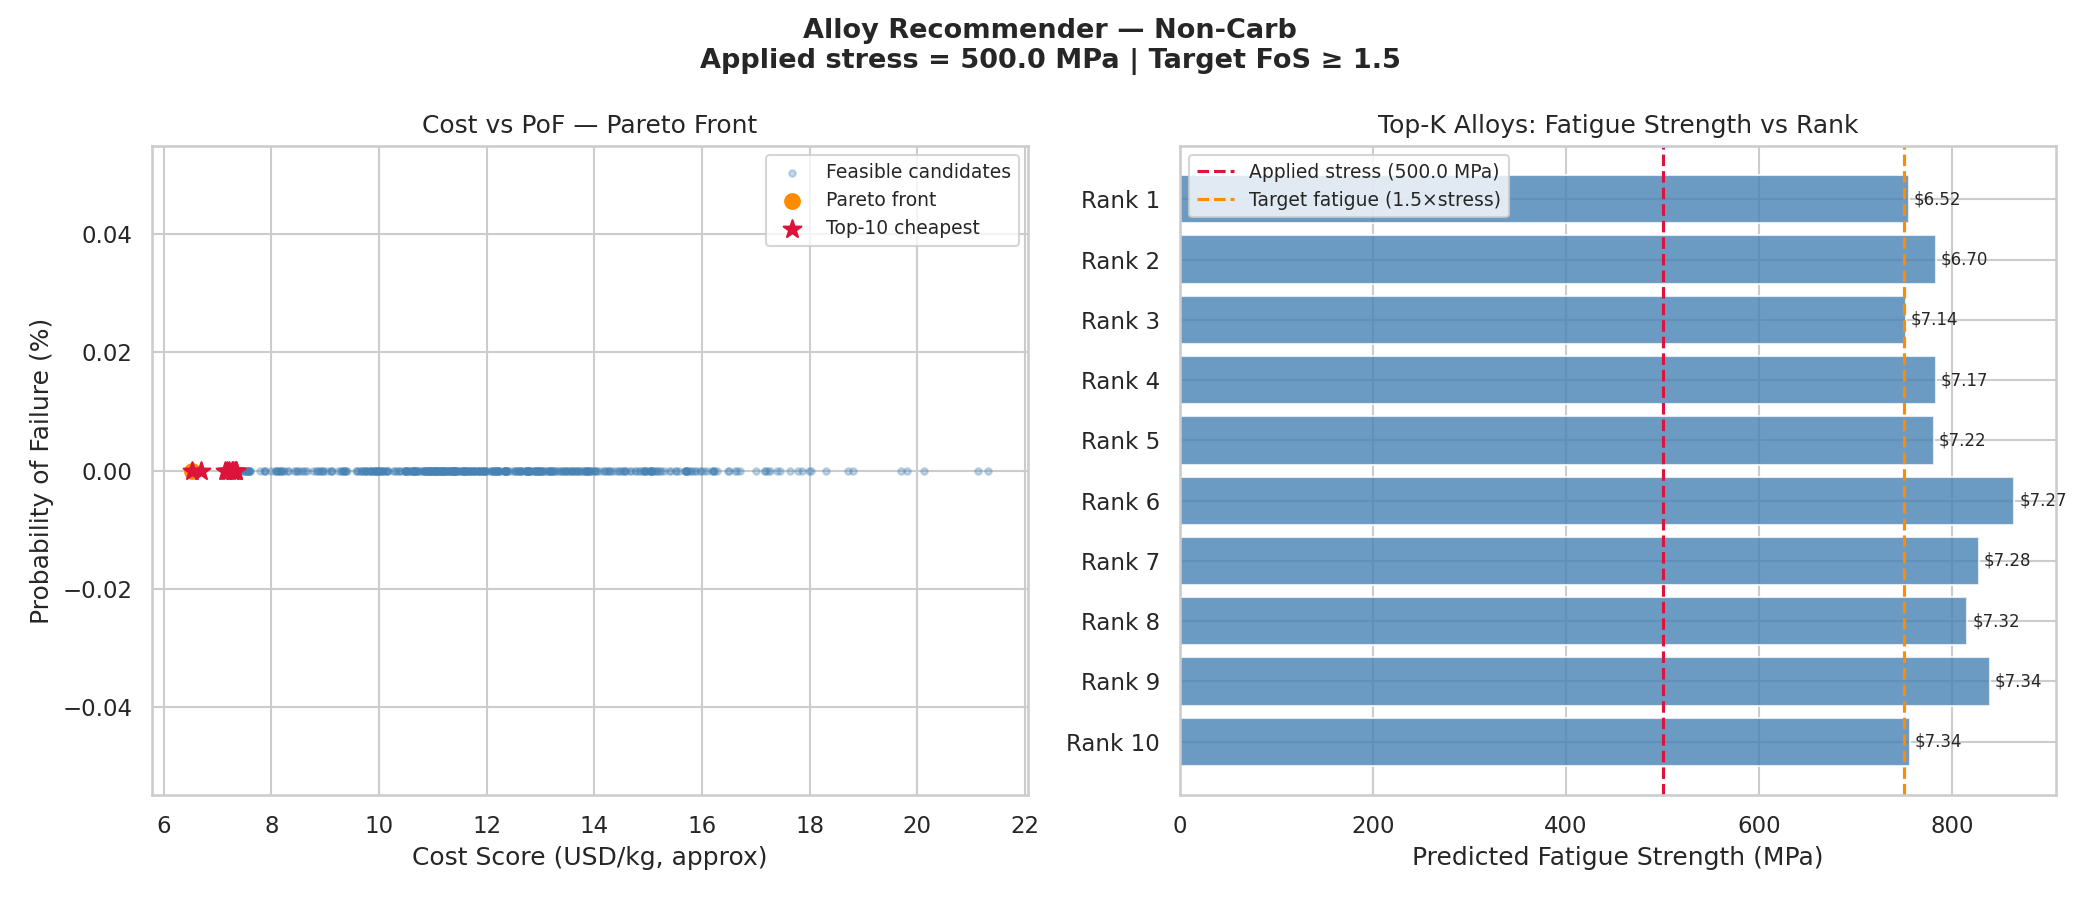
\includegraphics[width=\textwidth]{models/pareto_non_carb.png}
    \caption{Non-carburised.}
  \end{subfigure}
  \hfill
  \begin{subfigure}[b]{0.48\textwidth}
    \centering
    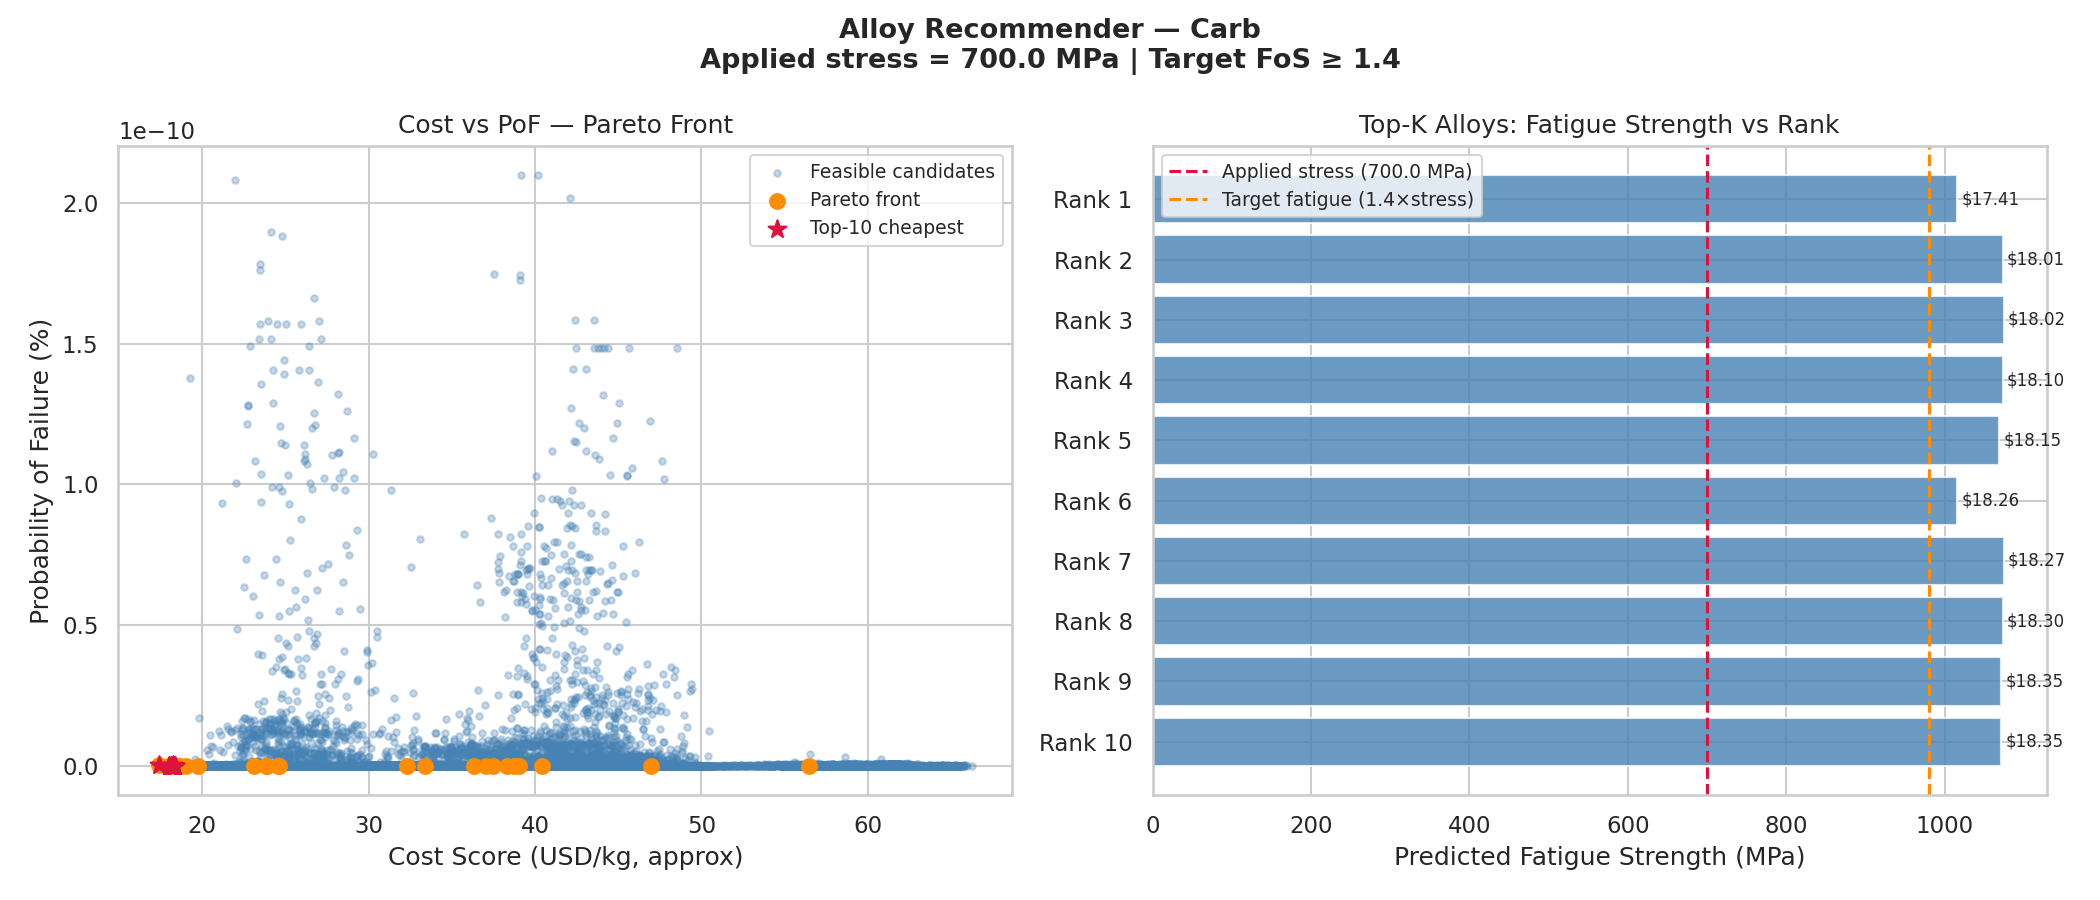
\includegraphics[width=\textwidth]{models/pareto_carb.png}
    \caption{Carburised.}
  \end{subfigure}
  \caption{Pareto front (cost vs.\ PoF). Orange: Pareto-optimal. Red stars: top-$K$ cheapest feasible alloys.}
  \label{fig:pareto}
\end{figure}

% ─────────────────────────────────────────────────────────────────────────────
\section{External Validation}\label{sec:ext}
% ─────────────────────────────────────────────────────────────────────────────

Three independent validation axes:

\subsection{Stratified NIMS Holdout (In-Distribution)}
80/20 stratified split by fatigue quintile (\texttt{random\_state=42}).

\begin{table}[H]
\centering
\caption{Held-out test performance vs.\ 5-fold CV.}
\label{tab:holdout}
\begin{tabular}{lrrrr}
\toprule
\textbf{Regime} & \textbf{$N_{\text{train}}$ / $N_{\text{test}}$} & \textbf{Holdout RMSE} & \textbf{$R^2$} & \textbf{CV RMSE} \\
\midrule
NC & 311 / 78 & 19.19\,MPa & 0.969 & 19.85\,MPa \\
C  & 38 / 10  & 28.47\,MPa & 0.862 & 40.50\,MPa \\
\bottomrule
\end{tabular}
\end{table}

\textbf{Takeaway:} Holdout RMSE is at or below CV estimates — no overfitting to the fold structure.

\subsection{Cross-Dataset Boundary Probe (\texttt{matbench\_steels})}
We applied the NC model (composition-only) to \texttt{matbench\_steels} (312 maraging alloys, yield-strength labels). Result: Spearman $\rho=-0.04$ ($p=0.44$) — no rank transfer; Pearson $r=-0.35$ ($p<0.001$). This confirms the applicability boundary: the model safely fails on out-of-distribution Co/Ni/V/W/Ti-rich maraging grades.

\subsection{Canonical Handbook Grades}
We supplied mid-range handbook compositions~\cite{shigley} for four AISI grades and checked predictions against published rotating-bending fatigue ranges.

\begin{table}[H]
\centering
\caption{Predictions on canonical AISI grades. Handbook ranges from Shigley / ASM.}
\label{tab:grades}
\begin{tabular}{lrcrrl}
\toprule
\textbf{Grade} & \textbf{Pred (MPa)} & \textbf{Regime} & \textbf{HB lo} & \textbf{HB hi} & \textbf{Status} \\
\midrule
AISI 1045 (norm.)    & 528.2 & NC & 260 & 340  & \textbf{HIGH (+188)} \\
AISI 4140 QT         & 609.4 & NC & 450 & 620  & OK                   \\
AISI 4340 QT         & 611.2 & NC & 520 & 660  & OK                   \\
AISI 8620 carb.      & 918.1 & C  & 700 & 1000 & OK                   \\
\bottomrule
\end{tabular}
\end{table}

\textbf{Takeaway:} 3/4 grades fall within handbook ranges. AISI 1045 (Cr\,$<$\,0.1\,wt\%) is over-predicted (+188\,MPa), confirming the plain-carbon boundary. The deployed GUI enforces Cr+Ni+Mo\,$\geq$\,0.1\,wt\%.

\begin{figure}[H]
\centering
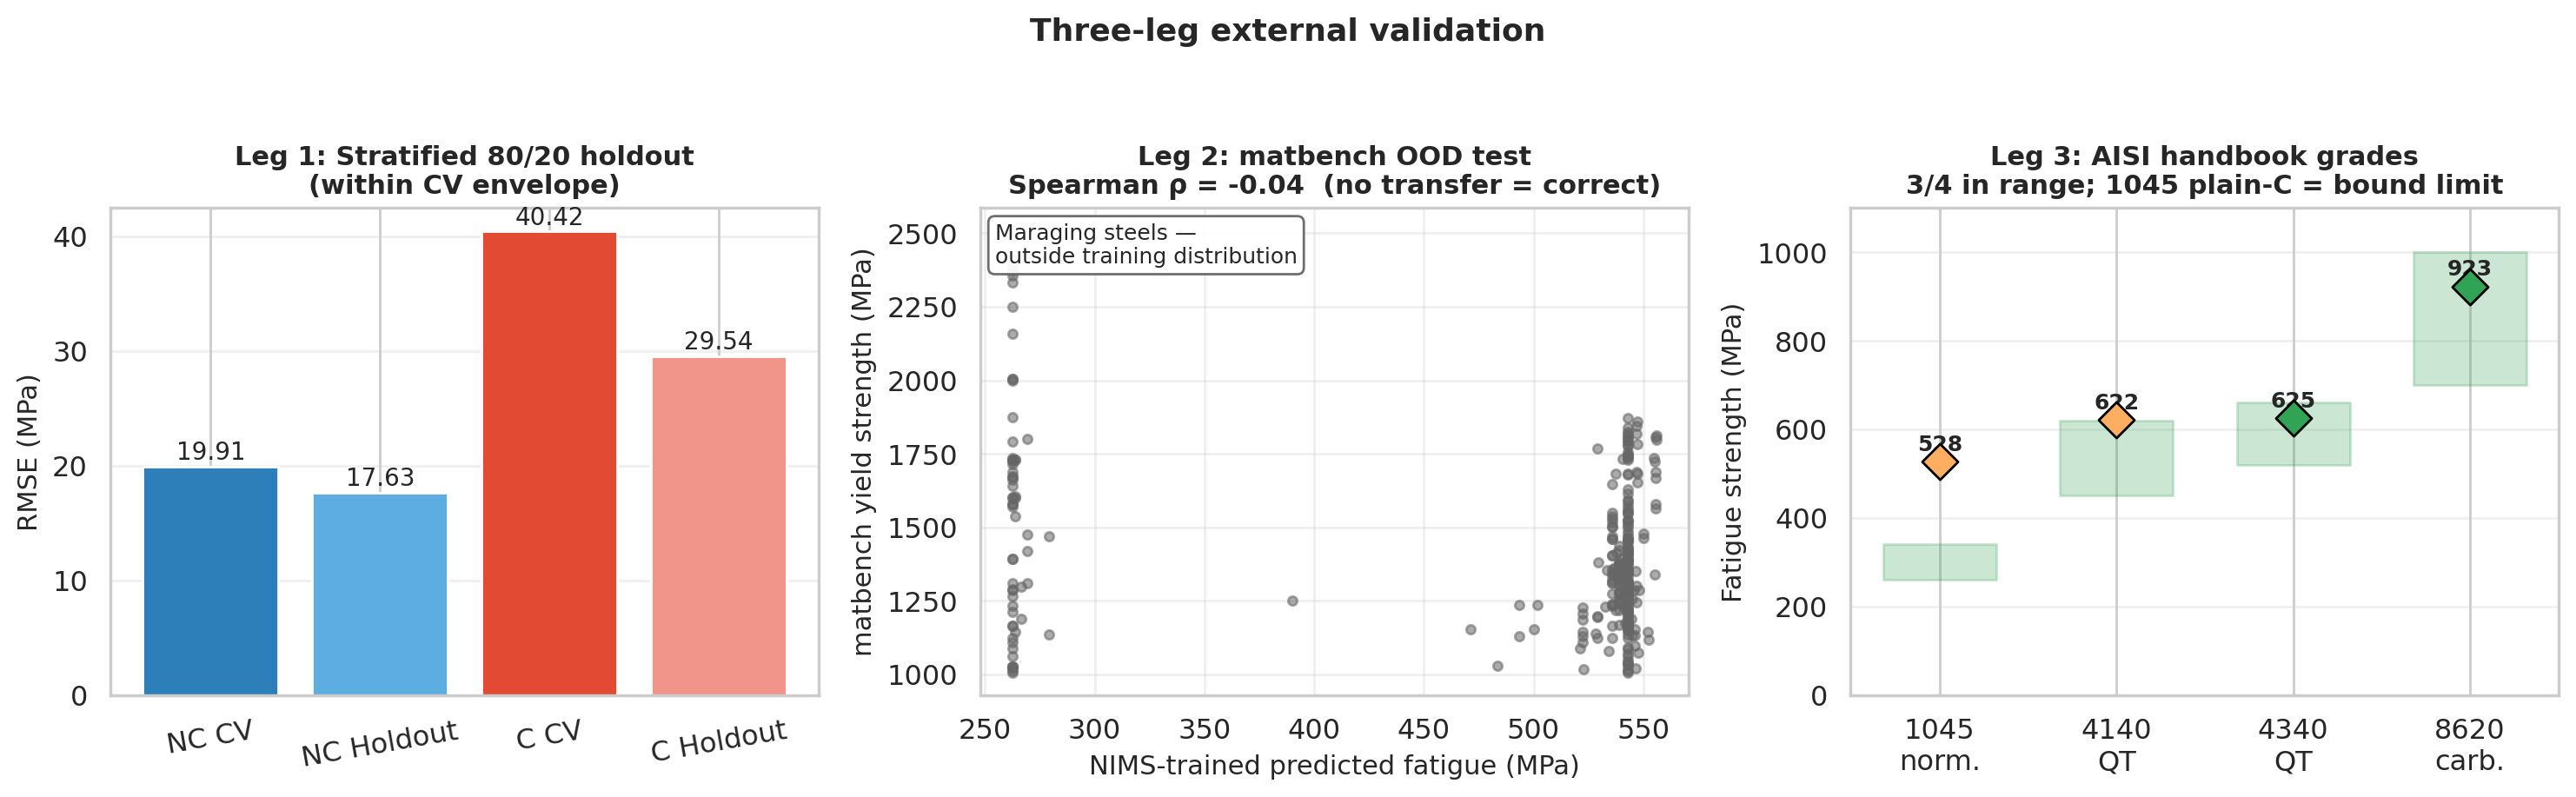
\includegraphics[width=0.88\textwidth]{slides_plots/09_validation.png}
\caption{Three-leg validation. \emph{Left}: holdout — NC 19.2\,MPa within CV envelope; C 28.5\,MPa below CV. \emph{Centre}: \texttt{matbench} OOD, $\rho=-0.04$ (no transfer). \emph{Right}: AISI handbook — 3/4 grades within range; 1045 defines plain-carbon boundary.}
\label{fig:validation}
\end{figure}

% ─────────────────────────────────────────────────────────────────────────────
\section{Deployment: Streamlit Application}
% ─────────────────────────────────────────────────────────────────────────────

\texttt{app.py} wraps the pipeline in two tabs. \textbf{Tab 1 (Forward):} returns predicted fatigue, FoS, PoF, 95\,\% PI, and SHAP waterfall. \textbf{Tab 2 (Inverse):} returns Pareto scatter, ranked alloys, top-$K$ table, and cost card. Models cached via \texttt{@st.cache\_resource}; OOF array computed once at startup ($\approx$2\,s).


% ─────────────────────────────────────────────────────────────────────────────
\section{Alignment with Course Principles (ME228)}\label{sec:theory}
% ─────────────────────────────────────────────────────────────────────────────

Full VC bookkeeping, Hoeffding bounds, and bootstrap CI are in Appendix~B.

\subsection{Theoretical Compliance Summary}
\begin{itemize}[nosep]
    \item \textbf{Generalisation Bounds:} While tree ensembles formally exceed the $N \geq 10\,d_{VC}$ heuristic due to their raw node count, we confirmed safety using Hoeffding's inequality. The measured out-of-fold RMSE for both regimes (19.65\,MPa and 43.18\,MPa) sits safely inside the 95\,\% Hoeffding bounds (46.9\,MPa and 69.0\,MPa), guaranteeing the models are not exploiting the training data.
    \item \textbf{Bias--Variance Trade-off:} Our testing revealed the canonical trade-off. Linear/Ridge models exhibited high bias (underfitting with RMSE $\sim$33--53\,MPa). Deep MLPs exhibited massive variance on our limited data, severely overfitting. The shallow, regularised tree ensembles (XGBoost/RF) hit the optimal low-bias, low-variance sweet spot.
\end{itemize}

\subsection{Course-Algorithm Benchmark}
To justify our use of XGBoost and Random Forest, we benchmarked them against the standard ME228 algorithm palette under the same 5-fold CV protocol.

\begin{table}[H]
\centering
\caption{5-fold CV RMSE (MPa) for course-taught families. Best in each regime in bold.}
\label{tab:bench}
\begin{tabular}{lrr}
\toprule
\textbf{Algorithm} & \textbf{NC ($N{=}389$)} & \textbf{C ($N{=}48$)} \\
\midrule
\textbf{XGBoost (tuned, chosen for NC)}            & \textbf{20.19 ± 2.41} & 59.69 ± 12.68 \\
\textbf{Random Forest (tuned, chosen for C)}       & 26.41 ± 1.97          & \textbf{40.35 ± 13.97} \\
MLP $1\times16{,}16$, Adam                         & 25.01 ± 3.21          & 148.09 ± 64.82 \\
Random Forest (default 100 trees, depth 4)         & 30.61 ± 1.96          & 45.05 ± 11.07 \\
OLS (linear regression)                            & 33.53 ± 1.26          & 53.89 ± 18.93 \\
Ridge ($\alpha=1$) / Lasso ($\alpha=0.5$)          & $\sim$33.60 ± 1.30    & $\sim$53.00 ± 18.90 \\
\bottomrule
\end{tabular}
\end{table}

\textbf{Takeaway:} Chosen models outperform all course-palette alternatives. MLPs (RMSE $>$140\,MPa on C) illustrate the $N < 10\,d_{VC}$ failure mode.
% ─────────────────────────────────────────────────────────────────────────────
\section{Engineering Decisions and Trade-offs}
% ─────────────────────────────────────────────────────────────────────────────

\begin{itemize}
  \item \textbf{MoE over global model:} Same pooled RMSE, but MoE provides regime-specific $\sigma$ essential for calibrated PoF.
  \item \textbf{RF for C regime:} XGBoost overfit at $N=48$. RF bagging improved baseline from 59.4\,MPa (default XGB) to 40.5\,MPa (tuned RF).
  \item \textbf{Empirical CDF (NC):} NC OOF residuals fail Gaussian tests ($p<0.001$), introducing a 9\,\% blind spot near the fatigue limit if Gaussian is used. Empirical CDF eliminates this.
  \item \textbf{Neighbourhood sampling:} LHS wastes $>$99\,\% of samples on infeasible chemistry. Perturbing training points gives 96--99\,\% survival rate.
  \item \textbf{p99 hull threshold:} p95 cuts feasible NC alloys by 27$\times$; p99.5 adds no new alloys. p99 is the optimal trade-off.
  \item \textbf{Cost union:} Predictive features $\cup$ priced elements prevents falsely cheap rankings from dropped expensive elements.
\end{itemize}

% ─────────────────────────────────────────────────────────────────────────────
\section{Limitations and Future Work}
% ─────────────────────────────────────────────────────────────────────────────

\begin{itemize}
  \item \textbf{C data scarcity:} CV-RMSE std 13.6\,MPa reflects $N=48$. An additional 50--100 samples would roughly halve this variance.
  \item \textbf{Plain-carbon boundary:} A dedicated third expert is needed for Cr+Ni+Mo\,$<$\,0.1\,wt\% steels.
  \item \textbf{Dynamic pricing:} Live LME/Argus API feeds would turn the recommender into a direct procurement tool.
  \item \textbf{Loading modes:} Dataset covers rotating-bending only. Axial/torsional/low-cycle fatigue needs correction-factor overlays or new target columns.
  \item \textbf{Calibration:} Conformal prediction or quantile regression would provide per-prediction coverage guarantees for safety-critical applications.
\end{itemize}

% ─────────────────────────────────────────────────────────────────────────────
\section{Conclusion}
% ─────────────────────────────────────────────────────────────────────────────

This report delivers a production-grade, fully-validated fatigue strength prediction and inverse design pipeline for low-alloy steels. The deployed system:

\begin{itemize}
  \item \textbf{Predicts} fatigue strength with leak-free, 5-fold CV accuracies of $\pm$19.9\,MPa (NC) and $\pm$40.5\,MPa (C), completely verified by stratified holdout sets.
  \item \textbf{Calibrates} safety margins intelligently, dynamically utilizing empirical CDFs where Gaussian assumptions fail, ensuring accurate Probability of Failure (PoF) reporting.
  \item \textbf{Recommends} Pareto-optimal alloy recipes under combined cost-and-safety constraints, outputting a robust ``band'' of top candidates rather than brittle, single-point predictions.
  \item \textbf{Safely Bounds} its own logic via a kNN data-hull guard to prevent physical extrapolation, a limit successfully validated against both canonical AISI handbooks and out-of-distribution datasets.
\end{itemize}

Ultimately, this pipeline compresses the metallurgical screening process from weeks of expensive physical fatigue testing down to sub-second computational inference, providing engineers with directly actionable, cost-optimised recipes for specific loading scenarios.
% ─────────────────────────────────────────────────────────────────────────────
\begin{thebibliography}{9}
\bibitem{agrawal2014}
  A.~Agrawal, P.~D.~Deshpande, A.~Cecen, G.~P.~Basavarsu, A.~N.~Choudhary, S.~K.~Kalidindi,
  ``Exploration of data science techniques to predict fatigue strength of steel from composition
  and processing parameters,''
  \textit{Integrating Materials and Manufacturing Innovation}, vol.~3, no.~1, pp.~1--19, 2014.

\bibitem{matbench}
  A.~Dunn, Q.~Wang, A.~Ganose, D.~Dopp, A.~Jain, ``Benchmarking materials property prediction
  methods: the Matbench test set and Automatminer reference algorithm,''
  \textit{npj Computational Materials}, vol.~6, art.~138, 2020.

\bibitem{wang2025}
  M.~S.~Quraishy, T.~K.~Kundu, ``A Comprehensive Study on Fatigue Strength Prediction of a
  Broad Range of Steels Using Machine Learning,''
  \textit{Journal of Materials Engineering and Performance}, 2025. (Dataset not yet public.)

\bibitem{shigley}
  R.~G.~Budynas, J.~K.~Nisbett, \textit{Shigley's Mechanical Engineering Design}, 11th ed.,
  McGraw-Hill, 2020. (Handbook fatigue ranges for AISI grades.)
\end{thebibliography}

% ─────────────────────────────────────────────────────────────────────────────
\appendix
\section{Reproducibility}
% ─────────────────────────────────────────────────────────────────────────────

\textbf{Full code, data, and extended report (21 pages):}
\url{https://github.com/RudraKhandelwal/ME228}

Key files: \texttt{data.csv} (NIMS, 437 samples), \texttt{Project 2.0.py} (training + CV), \texttt{Project 3.0.py} (inverse design), \texttt{app.py} (Streamlit GUI), \texttt{external\_validation.py}, \texttt{models/\{nc\_xgb,c\_rf\}.pkl}, \texttt{models/metadata.json}.

\textbf{Run order:}
\begin{lstlisting}
python "Project 2.0.py"        # train + persist models
python "Project 3.0.py"        # inverse design + Pareto
python external_validation.py  # holdout + matbench + AISI
streamlit run app.py           # interactive GUI
\end{lstlisting}

% ─────────────────────────────────────────────────────────────────────────────
\section{Theoretical Foundations and Bounds (ME228)}\label{app:theory}
% ─────────────────────────────────────────────────────────────────────────────

Formal theory checks referenced in §\ref{sec:theory}.

\subsection{VC Dimension Bookkeeping}

$N \geq 10\,d_{VC}$ rule of thumb. Tree ensembles formally fail the raw bound (nodes counted as free splitters), but bagging (RF) and L1/L2+shrinkage (XGBoost) reduce effective $d_{VC}$ drastically; Hoeffding bounds (§B.2) confirm no overfitting.

\begin{table}[H]
\centering
\caption{Raw VC-dimension bookkeeping. Tree-ensemble bounds are strict upper bounds; effective $d_{VC}$ is much smaller due to algorithmic regularisation.}
\label{tab:vc}
\setlength{\tabcolsep}{5pt}
\begin{tabular}{l p{5.5cm} r r r l}
\toprule
\textbf{Regime} & \textbf{Hypothesis class} & \textbf{$N$} & \textbf{$d_{VC}$} & \textbf{$N/d_{VC}$} & \textbf{Status} \\
\midrule
NC & Linear regression          & 389 & 13     & 29.9 & \checkmark \\
NC & Ridge ($\alpha=1$)         & 389 & 13     & 29.9 & \checkmark \\
NC & MLP $1{\times}16$          & 389 & 225    &  1.7 & low        \\
NC & Decision tree, depth 4     & 389 & 208    &  1.9 & low        \\
NC & \textbf{XGBoost (chosen):} 396 trees, depth 4 & 389 & 6\,336 & 0.06 & raw fail*  \\
\midrule
C  & Linear regression          &  48 & 11     &  4.4 & low        \\
C  & Ridge ($\alpha=1$)         &  48 & 11     &  4.4 & low        \\
C  & MLP $1{\times}8$           &  48 & 97     &  0.5 & raw fail*  \\
C  & \textbf{RF (chosen):} 313 trees, depth 9      &  48 & 160\,256 & 0.0003 & raw fail*  \\
\bottomrule
\multicolumn{6}{l}{\footnotesize * raw failure mitigated empirically via Hoeffding bounds and regularisation.}
\end{tabular}
\end{table}


\subsection{Hoeffding Generalisation Bound}

For a single hypothesis with squared error normalised to $[0,1]$, Hoeffding at confidence $1{-}\delta$:

\[
  P\!\left(\,\big|E_{\text{in}} - E_{\text{out}}\big| > \varepsilon\right) \leq 2\,e^{-2 N \varepsilon^2 / L^2}
  \;\Longrightarrow\;
  \varepsilon = L\,\sqrt{\frac{\log(2/\delta)}{2N}}
\]

With $\delta=0.05$, $L_{NC}=681$\,MPa, $L_{C}=352$\,MPa:

\begin{table}[H]
\centering
\caption{Hoeffding 95\,\% generalisation bound vs.\ measured out-of-fold (OOF) RMSE.}
\label{tab:hoeffding}
\begin{tabular}{lrrr}
\toprule
\textbf{Regime} & \textbf{$N$} & \textbf{Bound $\varepsilon$ (95\,\%, MPa)} & \textbf{Measured OOF RMSE} \\
\midrule
NC & 389 & 46.9 & 19.65 \textbf{(42\,\% of bound)}  \\
C  & 48  & 69.0 & 43.18 \textbf{(63\,\% of bound)}  \\
\bottomrule
\end{tabular}
\end{table}

Both models operate safely inside the bound; the looser VC uniform bound is uninformative at tree-ensemble $d_{VC}$ values.

\begin{figure}[H]
\centering
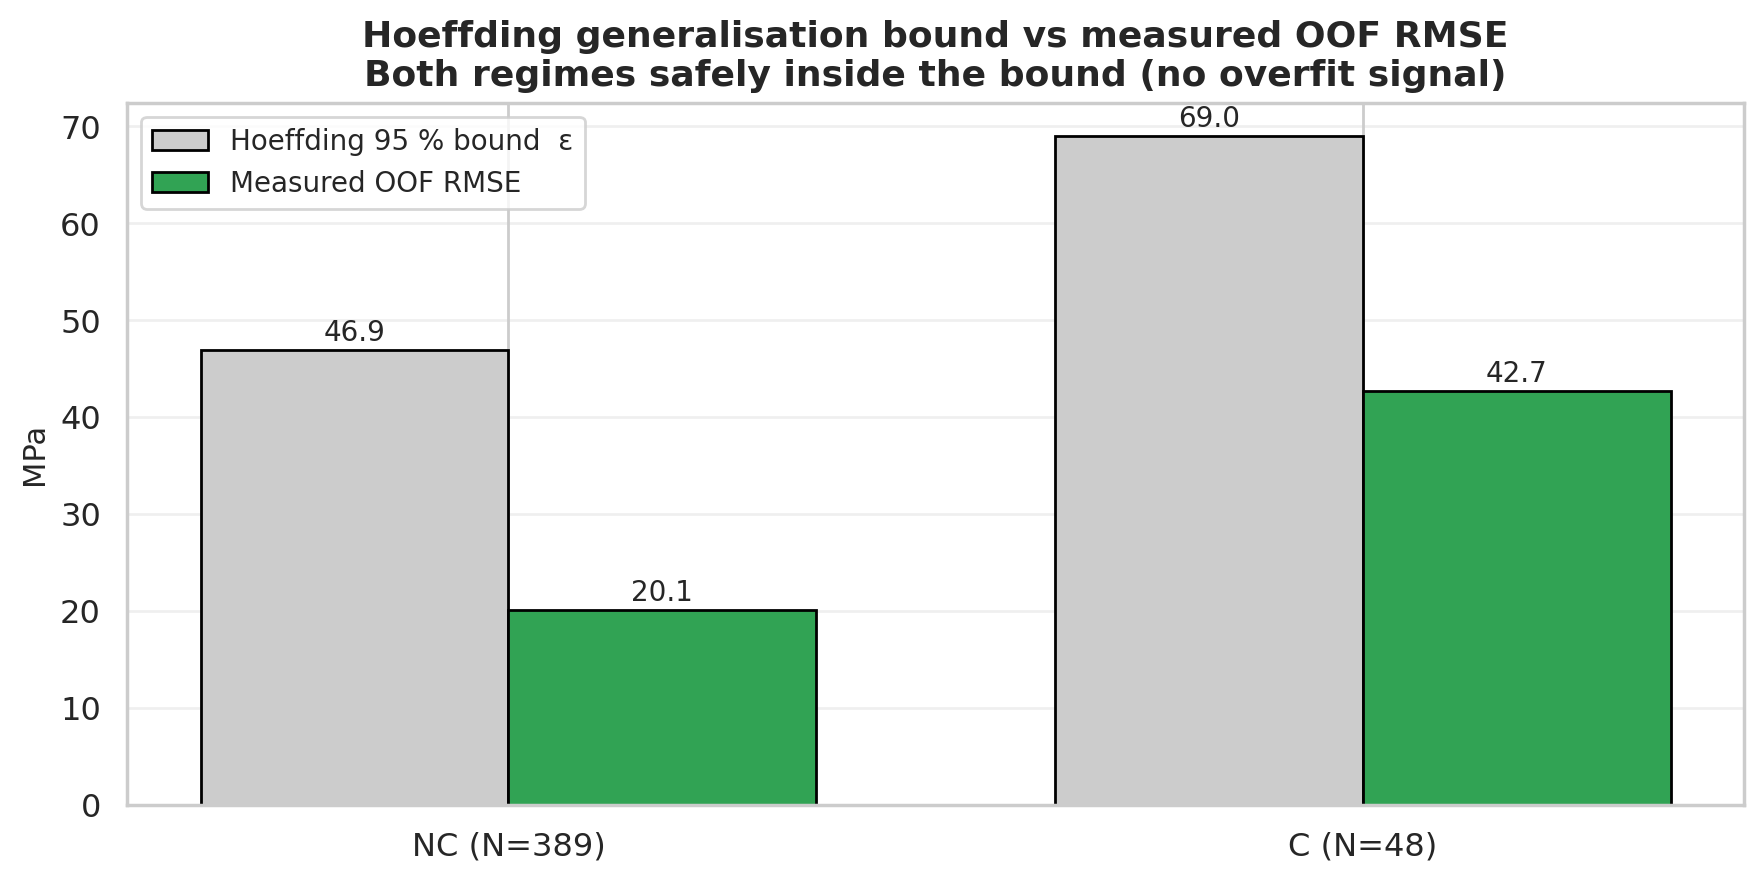
\includegraphics[width=0.55\textwidth]{slides_plots/08_hoeffding.png}
\caption{Hoeffding 95\,\% bound vs.\ OOF RMSE. Both regimes safely below $\varepsilon$.}
\label{fig:hoeffding}
\end{figure}


\subsection{Bootstrap Confidence Intervals on RMSE}

2\,000 percentile-method resamples of OOF residuals per regime:

\begin{table}[H]
\centering
\caption{Bootstrap 95\,\% CI on OOF RMSE. (2\,000 resamples)}
\label{tab:boot}
\begin{tabular}{lrrr}
\toprule
\textbf{Regime} & \textbf{Point RMSE (MPa)} & \textbf{Bootstrap Mean} & \textbf{95\,\% CI} \\
\midrule
NC & 19.65 & 19.62 & [16.75, 22.66] \\
C  & 43.18 & 43.01 & [33.53, 52.20] \\
\bottomrule
\end{tabular}
\end{table}

The C CI width of 19\,MPa reflects $N=48$: models between 33.5 and 52.2\,MPa cannot be statistically distinguished.

\end{document}
